Konstruieren Sie eine Reduktion
$\textsl{SUDOKU}\le_P\textsl{VERTEX-COLORING}$.

\begin{figure}
\begin{center}
\includeagraphics[width=0.25\hsize]{sudoku-1.pdf}
\end{center}
\caption{$2^2\times 2^2$-Sudoku zu Aufgabe \ref{70000028}
\label{70000028:sudoku}}
\end{figure}

\begin{hinweis}
Es reicht, die Reduktion für den Fall $n=2$ durchzuführen, also für
das $2^2\times 2^2$-Sudoku, wenn daraus klar
wird, wie die Verallgemeinerung für grössere $n$ zu handhaben ist.
Sie können ganz konkret das Beispiel aus Abbildung~\ref{70000028:sudoku}
für Ihre Konstruktion verwenden.
\end{hinweis}

\thema{polynomielle Reduktion}

\begin{loesung}
\definecolor{darkred}{rgb}{0.8,0,0}
\definecolor{darkgreen}{rgb}{0,0.6,0}
Zu einem Sudoku-Rätsel konstruieren wir einen Graphen wie folgt:
Jedes Feld des Sudoku-Rätsel wird zu einem Vertex des Graphen.
Der Graph erhält eine Kante für jedes Paar von Feldern, die nicht
das gleiche Zeichen enthalten dürfen, also wenn die beiden Felder in der
gleichen Zeile, der gleichen Spalte oder dem gleichen Unterfeld liegen.

Für ein $2^2\times 2^2$-Sudoku wie das in Abbildung~\ref{70000028:sudoku}
ergibt sich so der Graph:
\begin{equation}
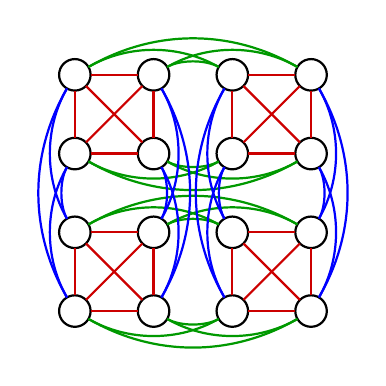
\begin{tikzpicture}[>=latex,thick]
\def\punkt#1#2{
	\draw (#1,#2) circle[radius=0.2];
}
\foreach \x in {0,...,3}{
	\foreach \y in {0,...,3}{
		\punkt{\x}{\y}
	}
}
\begin{scope}
\color{darkred}
\foreach \x in {0,2}{
	\foreach \y in {0,2}{
		\draw[shorten <= 0.2cm,shorten >= 0.2cm]
			(\x,\y) -- ({\x+1},{\y});
		\draw[shorten <= 0.2cm,shorten >= 0.2cm]
			(\x,{\y+1}) -- ({\x+1},{\y+1});
		\draw[shorten <= 0.2cm,shorten >= 0.2cm]
			({\x},\y) -- ({\x},{\y+1});
		\draw[shorten <= 0.2cm,shorten >= 0.2cm]
			({\x+1},\y) -- ({\x+1},{\y+1});

		\draw[shorten <= 0.2cm,shorten >= 0.2cm]
			(\x,\y) -- ({\x+1},{\y+1});
		\draw[shorten <= 0.2cm,shorten >= 0.2cm]
			({\x+1},\y) -- ({\x},{\y+1});
	}
}
\end{scope}

\begin{scope}
\color{darkgreen}
\draw[shorten <= 0.2cm,shorten >= 0.2cm] (0,0) to[out=-30,in=-150] (2,0);
\draw[shorten <= 0.2cm,shorten >= 0.2cm] (1,0) to[out=-30,in=-150] (2,0);
\draw[shorten <= 0.2cm,shorten >= 0.2cm] (1,0) to[out=-30,in=-150] (3,0);
\draw[shorten <= 0.2cm,shorten >= 0.2cm] (0,0) to[out=-30,in=-150] (3,0);
\draw[shorten <= 0.2cm,shorten >= 0.2cm] (0,2) to[out=-30,in=-150] (2,2);
\draw[shorten <= 0.2cm,shorten >= 0.2cm] (1,2) to[out=-30,in=-150] (2,2);
\draw[shorten <= 0.2cm,shorten >= 0.2cm] (1,2) to[out=-30,in=-150] (3,2);
\draw[shorten <= 0.2cm,shorten >= 0.2cm] (0,2) to[out=-30,in=-150] (3,2);
\draw[shorten <= 0.2cm,shorten >= 0.2cm] (0,1) to[out=30,in=150] (2,1);
\draw[shorten <= 0.2cm,shorten >= 0.2cm] (1,1) to[out=30,in=150] (2,1);
\draw[shorten <= 0.2cm,shorten >= 0.2cm] (1,1) to[out=30,in=150] (3,1);
\draw[shorten <= 0.2cm,shorten >= 0.2cm] (0,1) to[out=30,in=150] (3,1);
\draw[shorten <= 0.2cm,shorten >= 0.2cm] (0,3) to[out=30,in=150] (2,3);
\draw[shorten <= 0.2cm,shorten >= 0.2cm] (1,3) to[out=30,in=150] (2,3);
\draw[shorten <= 0.2cm,shorten >= 0.2cm] (1,3) to[out=30,in=150] (3,3);
\draw[shorten <= 0.2cm,shorten >= 0.2cm] (0,3) to[out=30,in=150] (3,3);
\end{scope}

\begin{scope}
\color{blue}
\draw[shorten <= 0.2cm,shorten >= 0.2cm] (0,0) to[out=120,in=-120] (0,3);
\draw[shorten <= 0.2cm,shorten >= 0.2cm] (0,0) to[out=120,in=-120] (0,2);
\draw[shorten <= 0.2cm,shorten >= 0.2cm] (0,1) to[out=120,in=-120] (0,2);
\draw[shorten <= 0.2cm,shorten >= 0.2cm] (0,1) to[out=120,in=-120] (0,3);
\draw[shorten <= 0.2cm,shorten >= 0.2cm] (2,0) to[out=120,in=-120] (2,3);
\draw[shorten <= 0.2cm,shorten >= 0.2cm] (2,0) to[out=120,in=-120] (2,2);
\draw[shorten <= 0.2cm,shorten >= 0.2cm] (2,1) to[out=120,in=-120] (2,2);
\draw[shorten <= 0.2cm,shorten >= 0.2cm] (2,1) to[out=120,in=-120] (2,3);

\draw[shorten <= 0.2cm,shorten >= 0.2cm] (1,0) to[out=60,in=-60] (1,3);
\draw[shorten <= 0.2cm,shorten >= 0.2cm] (1,0) to[out=60,in=-60] (1,2);
\draw[shorten <= 0.2cm,shorten >= 0.2cm] (1,1) to[out=60,in=-60] (1,2);
\draw[shorten <= 0.2cm,shorten >= 0.2cm] (1,1) to[out=60,in=-60] (1,3);
\draw[shorten <= 0.2cm,shorten >= 0.2cm] (3,0) to[out=60,in=-60] (3,3);
\draw[shorten <= 0.2cm,shorten >= 0.2cm] (3,0) to[out=60,in=-60] (3,2);
\draw[shorten <= 0.2cm,shorten >= 0.2cm] (3,1) to[out=60,in=-60] (3,2);
\draw[shorten <= 0.2cm,shorten >= 0.2cm] (3,1) to[out=60,in=-60] (3,3);


\end{scope}

\end{tikzpicture}
\label{70000028:graph}
\end{equation}
%\begin{equation}
%\entrymodifiers={++[o][F]}
%\xymatrix {
%{}\ar@{-}[r] \ar@{-}[d] \ar@{-}[dr]
%	\ar@/^10pt/@{-}[rr]
%	\ar@/^15pt/@{-}[rrr]
%	\ar@/_10pt/@{-}[dd]
%	\ar@/_15pt/@{-}[ddd]
%	&{} \ar@{-}[d]
%		\ar@{-}@/^2pt/[r]
%		\ar@{-}@/^10pt/[rr]
%		\ar@/^10pt/@{-}[dd]
%		\ar@/^15pt/@{-}[ddd]
%		&{}\ar@{-}[r] \ar@{-}[d] \ar@{-}[dr]
%			\ar@/_10pt/@{-}[dd]
%			\ar@/_15pt/@{-}[ddd]
%			\color{red}
%			&{} \ar@{-}[d]
%				\ar@/^10pt/@{-}[dd]
%				\ar@/^15pt/@{-}[ddd]
%				\color{red}
%\\
%{}\ar@{-}[r] \ar@{-}[ur]
%	\ar@/_10pt/@{-}[rr]
%	\ar@/_15pt/@{-}[rrr]
%	\ar@{-}@/_2pt/[d]
%	\ar@{-}@/_10pt/[dd]
%	&{}
%		\ar@{-}@/^2pt/[d]
%		\ar@{-}@/^10pt/[dd]
%		\ar@{-}@/_2pt/[r]
%		\ar@{-}@/_10pt/[rr]
%		&{}\ar@{-}[r] \ar@{-}[ur]
%			\ar@{-}@/_2pt/[d]
%			\ar@{-}@/_10pt/[dd]
%			&{}
%				\ar@{-}@/^2pt/[d]
%				\ar@{-}@/^10pt/[dd]
%\\
%{}\ar@{-}[r] \ar@{-}[d] \ar@{-}[dr]
%	\ar@/^10pt/@{-}[rr]
%	\ar@/^15pt/@{-}[rrr]
%	&{} \ar@{-}[d]
%		\ar@{-}@/^2pt/[r]
%		\ar@{-}@/^10pt/[rr]
%		&{}\ar@{-}[r] \ar@{-}[d] \ar@{-}[dr]
%			&{} \ar@{-}[d]
%\\
%{}\ar@{-}[r] \ar@{-}[ur]
%	\ar@/_10pt/@{-}[rr]
%	\ar@/_15pt/@{-}[rrr]
%	&{}
%		\ar@{-}@/_2pt/[r]
%		\ar@{-}@/_10pt/[rr]
%		&{}\ar@{-}[r] \ar@{-}[ur]
%			&{}
%}
%\label{70000028:graph}
%\end{equation}
Die roten Kanten stellen sicher, dass jedes Zeichen in einem Unterquadrat
nur einmal vorkommt.
Die grünen Kanten stellen zusätzlich sicher, dass in jeder Zeile jedes
Zeichen nur einmal vorkommt (die horizontalen roten Kanten sind dazu
ebenfalls nötig), während die vertikalen blauen Kanten erzwingen, dass
in jeder Spalte jedes Zeichen nur einmal vorkommt.

Ausserdem müssen wir die Vorgaben abbilden. Dazu konstruieren wir noch
zusätzliche Vertices, die wir mit den Zeichen aus $\Sigma$ anschreiben.
Wir nennen diese Vertizes die {\em Zeichenvertices}.
Die Vorgabefelder werden mit all den Zeichenvertices verbunden, die verschieden
sind vom Vorgabezeichen.
Für das $2^2\times 2^2$-Sudoku aus Abbildung \ref{70000028:sudoku}
müssen wir zum Graphen (\ref{70000028:graph}) noch die folgenden Kanten
hinzufügen:
\begin{equation}
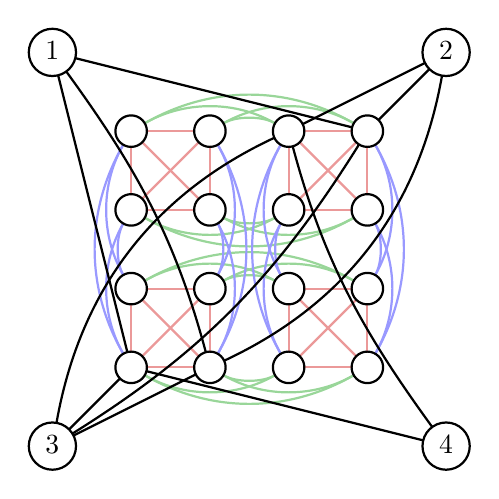
\begin{tikzpicture}[>=latex,thick]
\def\punkt#1#2{
	\draw (#1,#2) circle[radius=0.2];
}
\coordinate (q1) at (-1,4);
\coordinate (q2) at (4,4);
\coordinate (q3) at (-1,-1);
\coordinate (q4) at (4,-1);

\begin{scope}
\color{darkred!40}
\foreach \x in {0,2}{
	\foreach \y in {0,2}{
		\draw[shorten <= 0.2cm,shorten >= 0.2cm]
			(\x,\y) -- ({\x+1},{\y});
		\draw[shorten <= 0.2cm,shorten >= 0.2cm]
			(\x,{\y+1}) -- ({\x+1},{\y+1});
		\draw[shorten <= 0.2cm,shorten >= 0.2cm]
			({\x},\y) -- ({\x},{\y+1});
		\draw[shorten <= 0.2cm,shorten >= 0.2cm]
			({\x+1},\y) -- ({\x+1},{\y+1});

		\draw[shorten <= 0.2cm,shorten >= 0.2cm]
			(\x,\y) -- ({\x+1},{\y+1});
		\draw[shorten <= 0.2cm,shorten >= 0.2cm]
			({\x+1},\y) -- ({\x},{\y+1});
	}
}
\end{scope}

\begin{scope}
\color{darkgreen!40}
\draw[shorten <= 0.2cm,shorten >= 0.2cm] (0,0) to[out=-30,in=-150] (2,0);
\draw[shorten <= 0.2cm,shorten >= 0.2cm] (1,0) to[out=-30,in=-150] (2,0);
\draw[shorten <= 0.2cm,shorten >= 0.2cm] (1,0) to[out=-30,in=-150] (3,0);
\draw[shorten <= 0.2cm,shorten >= 0.2cm] (0,0) to[out=-30,in=-150] (3,0);
\draw[shorten <= 0.2cm,shorten >= 0.2cm] (0,2) to[out=-30,in=-150] (2,2);
\draw[shorten <= 0.2cm,shorten >= 0.2cm] (1,2) to[out=-30,in=-150] (2,2);
\draw[shorten <= 0.2cm,shorten >= 0.2cm] (1,2) to[out=-30,in=-150] (3,2);
\draw[shorten <= 0.2cm,shorten >= 0.2cm] (0,2) to[out=-30,in=-150] (3,2);
\draw[shorten <= 0.2cm,shorten >= 0.2cm] (0,1) to[out=30,in=150] (2,1);
\draw[shorten <= 0.2cm,shorten >= 0.2cm] (1,1) to[out=30,in=150] (2,1);
\draw[shorten <= 0.2cm,shorten >= 0.2cm] (1,1) to[out=30,in=150] (3,1);
\draw[shorten <= 0.2cm,shorten >= 0.2cm] (0,1) to[out=30,in=150] (3,1);
\draw[shorten <= 0.2cm,shorten >= 0.2cm] (0,3) to[out=30,in=150] (2,3);
\draw[shorten <= 0.2cm,shorten >= 0.2cm] (1,3) to[out=30,in=150] (2,3);
\draw[shorten <= 0.2cm,shorten >= 0.2cm] (1,3) to[out=30,in=150] (3,3);
\draw[shorten <= 0.2cm,shorten >= 0.2cm] (0,3) to[out=30,in=150] (3,3);
\end{scope}

\begin{scope}
\color{blue!40}

\draw[shorten <= 0.2cm,shorten >= 0.2cm] (0,0) to[out=120,in=-120] (0,3);
\draw[shorten <= 0.2cm,shorten >= 0.2cm] (0,0) to[out=120,in=-120] (0,2);
\draw[shorten <= 0.2cm,shorten >= 0.2cm] (0,1) to[out=120,in=-120] (0,2);
\draw[shorten <= 0.2cm,shorten >= 0.2cm] (0,1) to[out=120,in=-120] (0,3);
\draw[shorten <= 0.2cm,shorten >= 0.2cm] (2,0) to[out=120,in=-120] (2,3);
\draw[shorten <= 0.2cm,shorten >= 0.2cm] (2,0) to[out=120,in=-120] (2,2);
\draw[shorten <= 0.2cm,shorten >= 0.2cm] (2,1) to[out=120,in=-120] (2,2);
\draw[shorten <= 0.2cm,shorten >= 0.2cm] (2,1) to[out=120,in=-120] (2,3);

\draw[shorten <= 0.2cm,shorten >= 0.2cm] (1,0) to[out=60,in=-60] (1,3);
\draw[shorten <= 0.2cm,shorten >= 0.2cm] (1,0) to[out=60,in=-60] (1,2);
\draw[shorten <= 0.2cm,shorten >= 0.2cm] (1,1) to[out=60,in=-60] (1,2);
\draw[shorten <= 0.2cm,shorten >= 0.2cm] (1,1) to[out=60,in=-60] (1,3);
\draw[shorten <= 0.2cm,shorten >= 0.2cm] (3,0) to[out=60,in=-60] (3,3);
\draw[shorten <= 0.2cm,shorten >= 0.2cm] (3,0) to[out=60,in=-60] (3,2);
\draw[shorten <= 0.2cm,shorten >= 0.2cm] (3,1) to[out=60,in=-60] (3,2);
\draw[shorten <= 0.2cm,shorten >= 0.2cm] (3,1) to[out=60,in=-60] (3,3);

\end{scope}

\foreach \x in {0,...,3}{
	\foreach \y in {0,...,3}{
		\punkt{\x}{\y}
	}
}


\draw (q1) circle[radius=0.3];
\draw (q2) circle[radius=0.3];
\draw (q3) circle[radius=0.3];
\draw (q4) circle[radius=0.3];

\node at (q1) {$1\mathstrut$};
\node at (q2) {$2\mathstrut$};
\node at (q3) {$3\mathstrut$};
\node at (q4) {$4\mathstrut$};

\draw[shorten <= 0.3cm,shorten >= 0.2cm] (q1) -- (3,3);
\draw[shorten <= 0.3cm,shorten >= 0.2cm] (q1) -- (0,0);
\draw[shorten <= 0.3cm,shorten >= 0.2cm]
	(q1) to[out=-54,in=105] (1,0);

\draw[shorten <= 0.3cm,shorten >= 0.2cm] (q2) -- (3,3);
\draw[shorten <= 0.3cm,shorten >= 0.2cm] (q2) -- (2,3);
\draw[shorten <= 0.3cm,shorten >= 0.2cm]
	(q2) to[out=-100,in=25] (1,0);

\draw[shorten <= 0.3cm,shorten >= 0.2cm] (q3) -- (0,0);
\draw[shorten <= 0.3cm,shorten >= 0.2cm] (q3) -- (1,0);
\draw[shorten <= 0.3cm,shorten >= 0.2cm]
	(q3) to[out=80,in=-155] (2,3);
\draw[shorten <= 0.3cm,shorten >= 0.2cm]
	(q3) to[out=32,in=-122] (3,3);

\draw[shorten <= 0.3cm,shorten >= 0.2cm] (q4) -- (0,0);
\draw[shorten <= 0.3cm,shorten >= 0.2cm]
	(q4) to[out=126,in=-75] (2,3);


\end{tikzpicture}
\label{70000028:vorgaben}
\end{equation}
%\begin{equation}
%\entrymodifiers={++[o][F]}
%\xymatrix {
%{1}
%	&*+\txt{}
%		&*+\txt{}
%			&*+\txt{}
%				&*+\txt{}
%					&{2}
%\\
%*+\txt{}
%	&{}%\ar@{-}[r] \ar@{-}[d] \ar@{-}[dr]
%		%\ar@/^10pt/@{-}[rr]
%		%\ar@/^15pt/@{-}[rrr]
%		%\ar@/_10pt/@{-}[dd]
%		%\ar@/_15pt/@{-}[ddd]
%		&{} %\ar@{-}[d]
%			%\ar@{-}@/^2pt/[r]
%			%\ar@{-}@/^10pt/[rr]
%			%\ar@/^10pt/@{-}[dd]
%			%\ar@/^15pt/@{-}[ddd]
%			&{}%\ar@{-}[r] \ar@{-}[d] \ar@{-}[dr]
%				%\ar@/_10pt/@{-}[dd]
%				%\ar@/_15pt/@{-}[ddd]
%				\ar@{-}[urr]
%				\ar@{-}@/_9pt/[ddddrr]
%				\ar@{-}@/_25pt/[ddddlll]
%				&{} %\ar@{-}[d]
%					%\ar@/^10pt/@{-}[dd]
%					%\ar@/^15pt/@{-}[ddd]
%					\ar@{-}[ullll]
%					\ar@{-}[ur]
%					\ar@{-}@/^12pt/[ddddllll]
%					&*+\txt{}
%\\
%*+\txt{}
%	&{}%\ar@{-}[r] \ar@{-}[ur]
%		%\ar@/_10pt/@{-}[rr]
%		%\ar@/_15pt/@{-}[rrr]
%		%\ar@{-}@/_2pt/[d]
%		%\ar@{-}@/_10pt/[dd]
%		&{}
%			%\ar@{-}@/^2pt/[d]
%			%\ar@{-}@/^10pt/[dd]
%			%\ar@{-}@/_2pt/[r]
%			%\ar@{-}@/_10pt/[rr]
%			&{}%\ar@{-}[r] \ar@{-}[ur]
%				%\ar@{-}@/_2pt/[d]
%				%\ar@{-}@/_10pt/[dd]
%				&{}
%					%\ar@{-}@/^2pt/[d]
%					%\ar@{-}@/^10pt/[dd]
%					&*+\txt{}
%\\
%*+\txt{}
%	&{}%\ar@{-}[r] \ar@{-}[d] \ar@{-}[dr]
%		%\ar@/^10pt/@{-}[rr]
%		%\ar@/^15pt/@{-}[rrr]
%		&{} %\ar@{-}[d]
%			%\ar@{-}@/^2pt/[r]
%			%\ar@{-}@/^10pt/[rr]
%			&{}%\ar@{-}[r] \ar@{-}[d] \ar@{-}[dr]
%				&{} %\ar@{-}[d]
%					&*+\txt{}
%\\
%*+\txt{}
%	&{}%\ar@{-}[r] \ar@{-}[ur]
%		%\ar@/_10pt/@{-}[rr]
%		%\ar@/_15pt/@{-}[rrr]
%		\ar@{-}[uuuul]
%		\ar@{-}[dl]
%		\ar@{-}[drrrr]
%		&{}
%			%\ar@{-}@/_2pt/[r]
%			%\ar@{-}@/_10pt/[rr]
%			\ar@{-}@/_9pt/[uuuull]
%			\ar@{-}@/_25pt/[uuuurrr]
%			\ar@{-}[dll]
%			&{}%\ar@{-}[r] \ar@{-}[ur]
%				&{}
%					&*+\txt{}
%\\
%{3}
%	&*+\txt{}
%		&*+\txt{}
%			&*+\txt{}
%				&*+\txt{}
%					&{4}
%}
%\label{70000028:vorgaben}
%\end{equation}
Um sicherzustellen, dass diese neuen Knoten verschiedene Farbe erhalten,
müssen diese untereinander alle verbunden werden, sie müssen also
einen vollständigen Teilgraphen bilden.
Diese Verbindungen sind der Übersichtlichkeit halber nicht eingezeichnet.

Die Vereinigung der Kanten in (\ref{70000028:graph}) und
(\ref{70000028:vorgaben}) liefert den Graphen, der dem gegebenen
Sudoku-Rätsel zugeordnet wird.
Für die Zahl der Farben setzen wir $k=|\Sigma|$, im Beispiel des
$2^2\times 2^2$-Sudokus aus Abbildung~\ref{70000028:sudoku} ist $k=4$.

Ist das Sudoku-Rätsel lösbar, kann man eine beliebige
Zuordnung von Farben zu den einzelnen Zeichen von $\Sigma$ verwenden,
um die Vertizes des Graphen einzufärben. 

Ist umgekehrt der konstruierte Graph mit $k$ Farben einfärbbar, dann kann man
die Farben der Zeichen-Vertizes verwenden, um allen anderen Vertizes
ebenfalls ein Zeichen zuzuordnen. Diese Zeichenbelegung ist automatisch
eine Lösung. Die Kanten innerhalb des Sudoku-Feldes sorgen dafür, dass
die Sudoku-Regeln eingehalten werden, die Kanten zu den Zeichen-Vertizes
sorgen dafür, dass die Vorgaben erfüllt sind.

Wir haben damit gezeigt, dass der konstruierte Graph genau dann mit
$k$ Farben einfärbbar ist, wenn das Sudoku-Rätsel lösbar ist. 
Ausserdem ist der Aufwand für die Konstruktion des Graphen von der
Grössenordnung des ursprünglichen Sudoku, also $O(n)$. Die konstruierte
Reduktion ist also sogar eine polynomielle Reduktion.
\end{loesung}


